% \IUref{IUAdmPS}{Administrar Planta de Selección}
% \IUref{IUModPS}{Modificar Planta de Selección}
% \IUref{IUEliPS}{Eliminar Planta de Selección}

%-------------------------------------- TERMINA descripción del caso de uso.

%\begin{UseCase}[archivo de imágen]{UCX}{Nombre del Caso de uso}{
	\begin{UseCase}{CU9.0}{Actualizar datos de área}{
		En esta sección el gerente o la recepcionista podrán modificar los datos del área que se registró, con el propósito de hacer los cambios pertinentes en la información que describe el área, con el fin de corregir errores o modificaciones en el área.
	}
		\UCitem{Versión}{1.0}
		\UCitem{Actor}{Gerente}
		\UCitem{Propósito}{Hacer cambios en la imformación que describe el área, con la intención de 			corregir errores o modificaciones en el área.}
		\UCitem{Entradas}{Nombre del Área, Tipo de área, largo, ancho, capacidad, responsable y 					     descripción.}
		\UCitem{Origen}{Los datos serán digitados desde el teclado.}
		\UCitem{Salidas}{Mensaje de que los datos han sido modificados correctamente.}
		\UCitem{Destino}{Los nuevos registros se verán reflejados en la base de datos.}
		\UCitem{Precondiciones}{Que el área se encuentre registrada previamente.}
		\UCitem{Postcondiciones}{El área registrada se verá reflejada en la sección de consultas.}
		\UCitem{Errores}{Que el sistema no efectué la operación requerida.
		Que los datos ingresados no correspondan al tipo de dato que se pide.}
		\UCitem{Tipo}{Caso de uso primario.}
		\UCitem{Observaciones}{}
		\UCitem{Autor}{Francisco García Enríquez.}
		\UCitem{Revisor}{Martin Carrillo.}
	\end{UseCase}


	\begin{UCtrayectoria}{Principal}
		\UCpaso[\UCactor] Selecciona del menú principal la opción Áreas.
		\UCpaso Muestra las opciones que el gerente pueda realizar: Registrar Áreas, Consultar Áreas, Eliminar Áreas, Dar de Baja Áreas y Actualizar Áreas.
		\UCpaso[\UCactor] Selecciona la opción de actualizar datos.
		\UCpaso Mostrará el formulario para registrar un área.		
		\UCpaso[\UCactor] Ingresará el nombre del área.
		\UCpaso[\UCactor] Confirma el registro presionando el botón de registrar.
		\UCpaso Muestra el mensaje {\bf MSG9-}``largo, ancho y responsable deben ser ingresados.'' 	
		\UCpaso[\UCactor] Ingresa caracteres en el campo largo y confirma el envio.
		\UCpaso Muestra un mensaje {\bf MSG10-}``campo largo debe ser numérico''
		\UCpaso Se queda en el campo largo para ingresar el dato correcto.
		\UCpaso[\UCactor] Confirma el registro y presiona el botón registrar.
		\UCpaso Manda un mensaje de error {\bf MSG11-}``el campo ancho debe ser ingresado''.
		\UCpaso devuelve el focus al campo ancho para corregir el dato.
		\UCpaso[\UCactor] Ingresa en el campo ancho un carácter como registro.
		\UCpaso[\UCactor] Confirma el registro presionando el botón registrar.
		\UCpaso Le manda un mensaje de error, {\bf MSG12-}``campo ancho debe ser numérico''.
		\UCpaso[\UCactor] Ingresa un dato numérico en el campo ancho.
		\UCpaso[\UCactor] Confirma el registro presionando el botón  de registrar área.
		\UCpaso Le manda un mensaje de error, {\bf MSG13-}``el campo responsable debe ser ingresado''.
		\UCpaso[\UCactor] Ingresa un dato numérico en el campo responsable.
		\UCpaso le manda un mensaje de error, {\bf MSG14-}``el campo responsable solo acepta letras y espacios en blanco''. 
		\UCpaso[\UCactor] Ingresa letras y espacios en blanco en el campo responsable.
		\UCpaso[\UCactor] Confirma el registro, presionando el botón de registrar área.
		\UCpaso Muestra una pantalla con un mensaje, {\bf MSG15-}``el registro fue exitoso''.
	\end{UCtrayectoria}
		
		\begin{UCtrayectoriaA}{A}{El gerente no llena la información con el tipo de dato correspondiente.}
			\UCpaso[\UCactor] Introduce espacios en blanco al inicio o caracteres especiales asi como datos numericos en el campo nombre.
			\UCpaso[\UCactor] Confirma el registro y presiona el boton registrar.
			\UCpaso Mostrará un mensaje  {\bf MSG16-}``el campo solo acepta letras y espacios en blanco''.
			\UCpaso[] Termina el caso de uso.
		\end{UCtrayectoriaA}

\begin{figure}[htbp!]
		\centering
			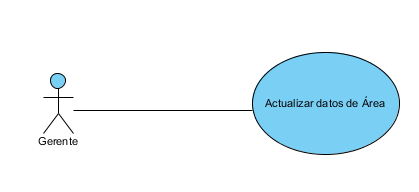
\includegraphics[width=0.8\textwidth]{images/ActualizarArea}
		\caption{Diagrama de Casos de Uso del sistema.}
	\end{figure}